%!TEX root = ../thesis.tex
% ******************************* Thesis Appendix B ********************************

\chapter{Supplementary Figures}

\section{Additional results for Chapter 3}

\begin{figure}[h]
    \centering
    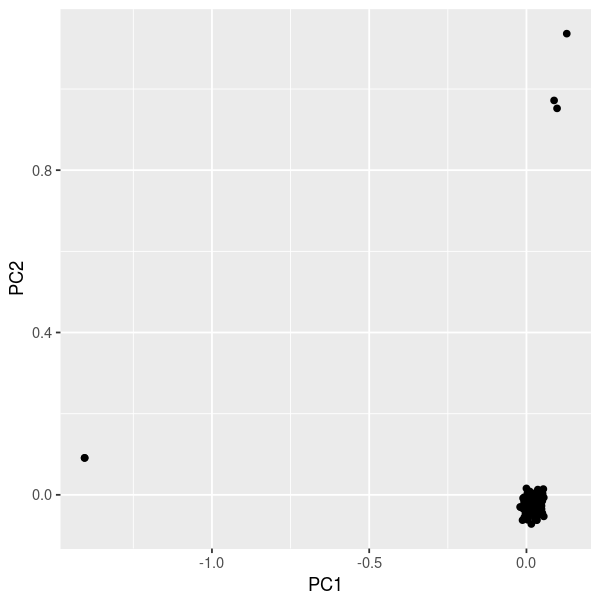
\includegraphics[width=10cm]{Appendix2/Fig/supplement_genotype_pcs.png}
    \caption[Population structure of donors included in the study]{\textbf{Population structure of donors included in the study.} \\
    Principal component (PC) decomposition of the kinship matrix (calculated using PLINK \cite{purcell2007plink}) across all cell lines included in our study.
    The four outlier cell lines were excluded from the analyses described in \textbf{section \ref{sec:best_practice}}.}
    \label{suppl_fig:kinship_pcs}
\end{figure}

\begin{figure}[h]
    \centering
    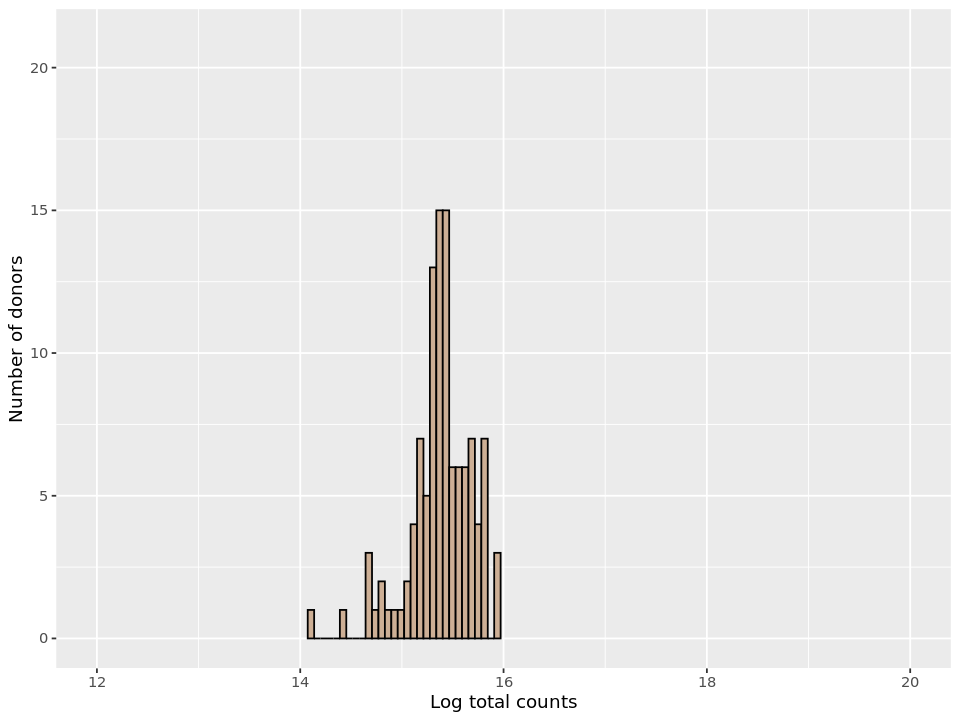
\includegraphics[width=12cm]{Appendix2/Fig/suppl_distribution_fixed_ncells.png}
    \caption[Distribution of total reads scRNA-seq same number of cells per donor]{Distribution of total reads from a scRNA-seq dataset, when considering the same number of cells for each donor.
    Same as the left panel from \textbf{Fig. \ref{fig:sc_bulk_counts}}, but downsampling to the same number of cells (n=10) from each donor.}
    \label{suppl_fig:counts_sc_ncells}
\end{figure}

\begin{figure}[h]
    \centering
    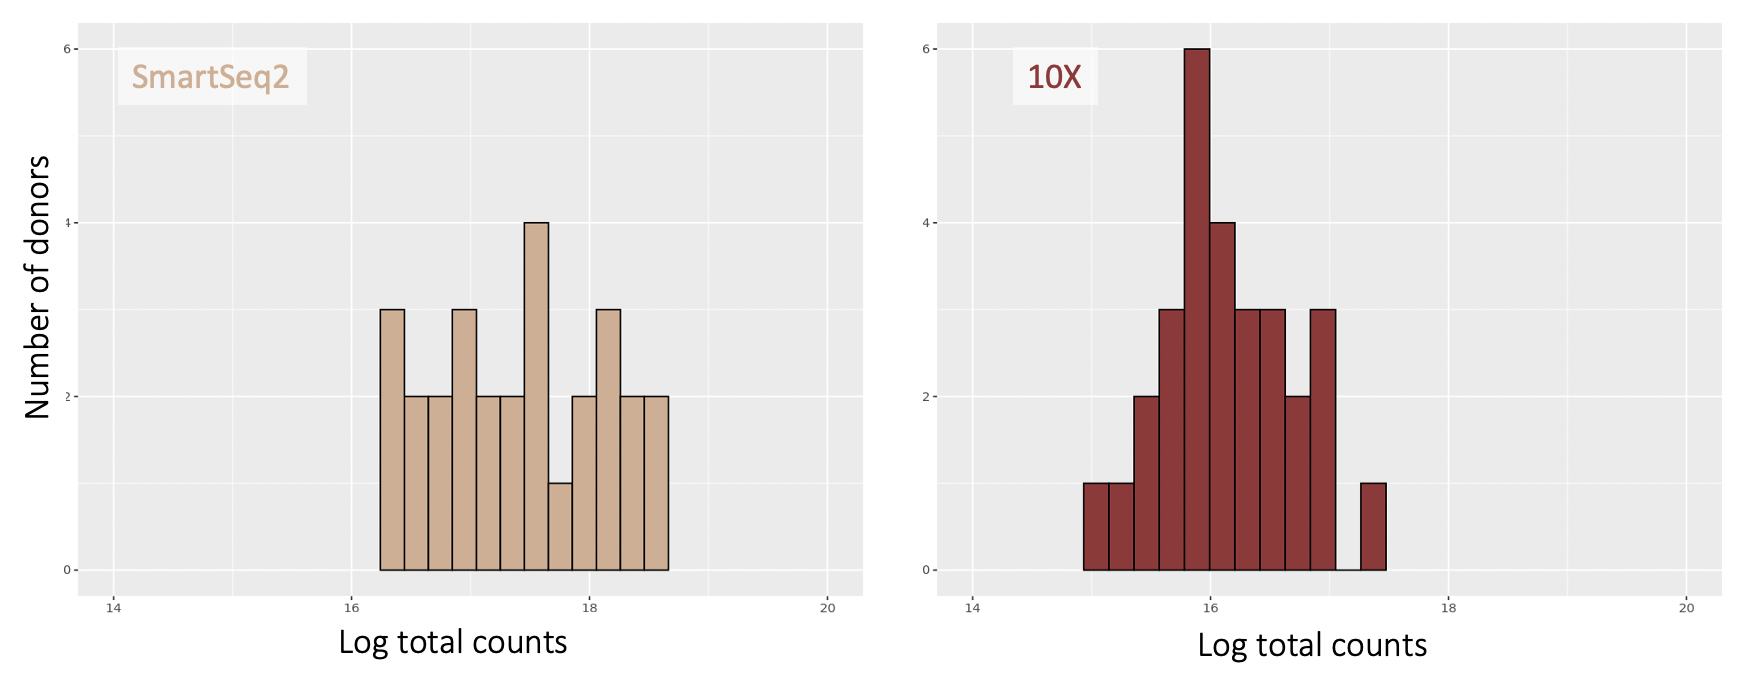
\includegraphics[width=15cm]{Appendix2/Fig/suppl_distribution_10x_ss2.png}
    \caption[Distribution of total reads between scRNA-seq technologies]{Distribution of total reads between scRNA-seq technologies, when considering the same 29 lines.
    Similar to \textbf{Fig. \ref{fig:sc_bulk_counts}}, but considering SmartSeq2 and 10x data from the same 29 cell lines.}
    \label{suppl_fig:counts_sc_technologies}
\end{figure}

\begin{figure}[h]
    \centering
    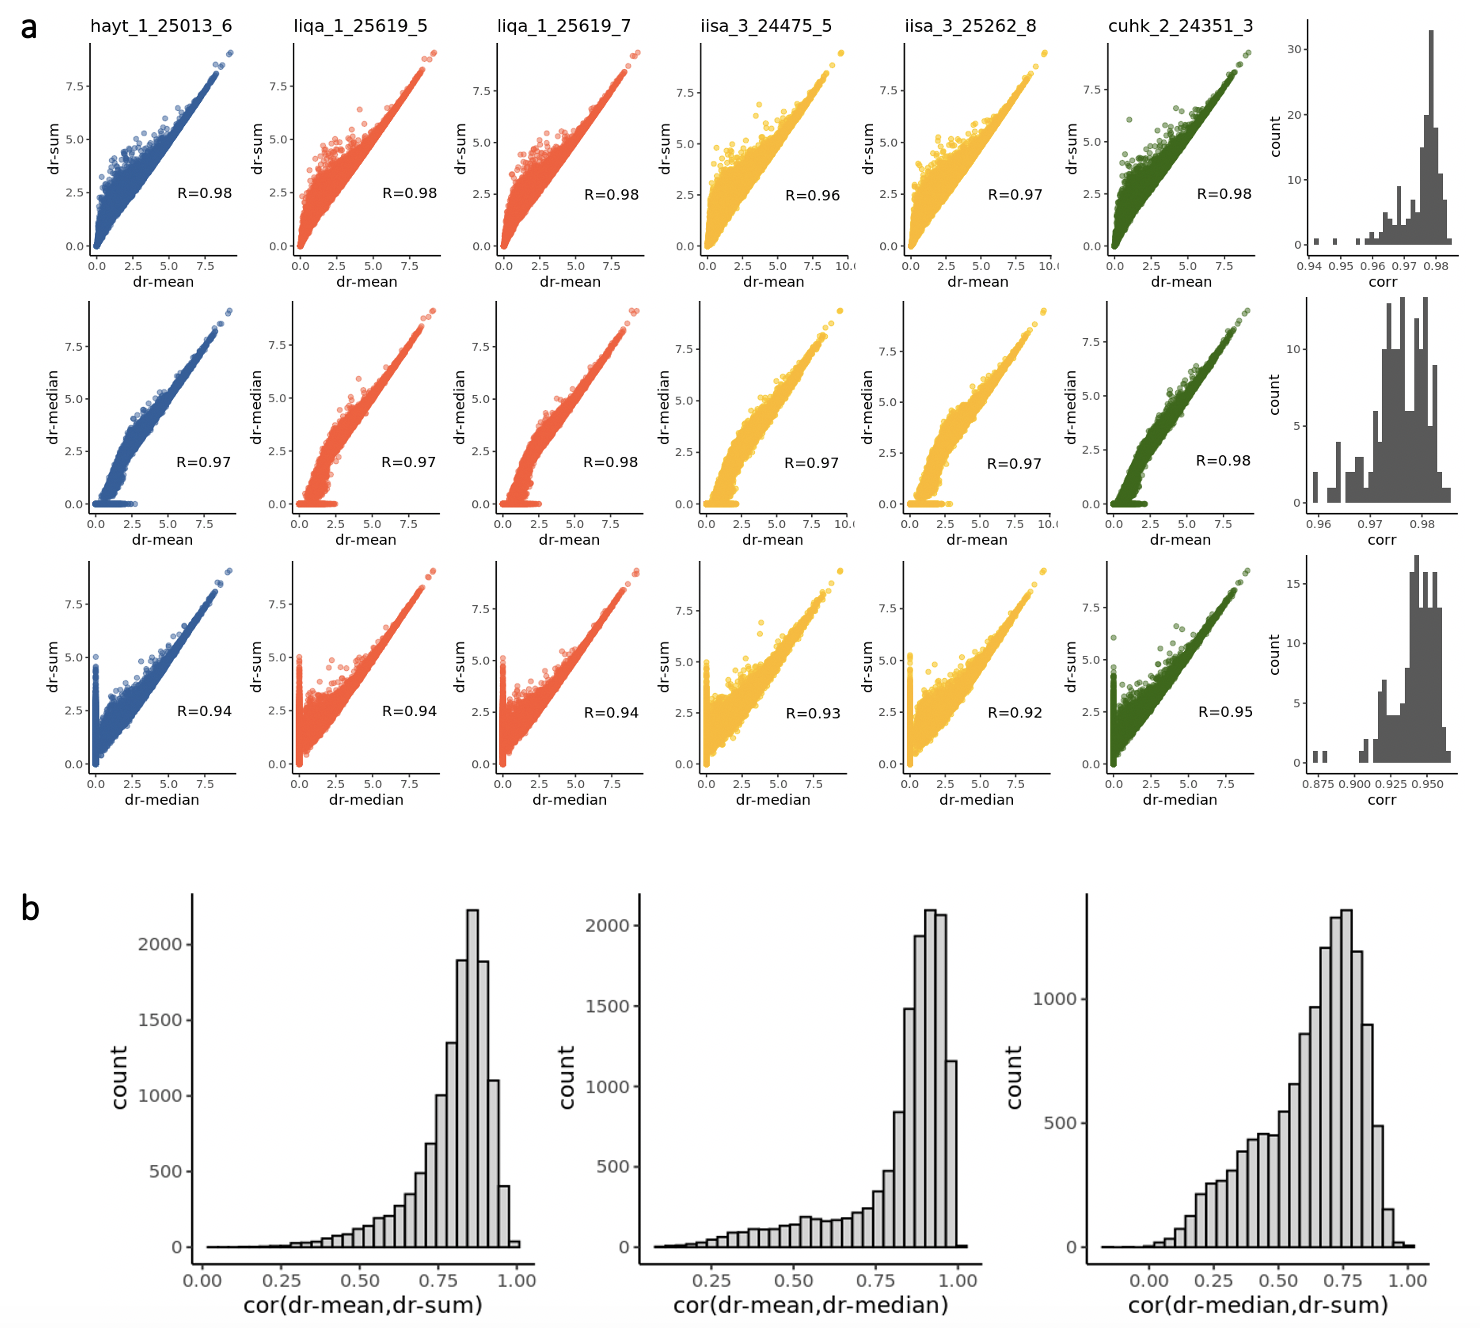
\includegraphics[width=15cm]{Appendix2/Fig/supp_aggregated_figures_dr.png}
    \caption[Comparison of `dr' aggregated measures]{\textcolor{blue}{\textbf{Comparison of `dr' aggregated measures.}\\
    (a) For a random selection of 4 donors (two of which present in two sequencing runs, resulting in 6 donor-run combinations, or samples), scatter plots between aggregation metrics, across the set of common genes (n=12,720).
    First row is dr-mean vs dr-sum, second dr-mean vs dr-median, third dr-median vs dr-sum.
    The last column represents, for each of the comparisons a histogram of the distribution of correlations, across donors.
    (b) Histograms representing the distribution of correlations across donors, for each genes, for the same three comparisons as in (a).}}
    \label{suppl_fig:aggregation_comparison_dr}
\end{figure}

\begin{figure}[h]
    \centering
    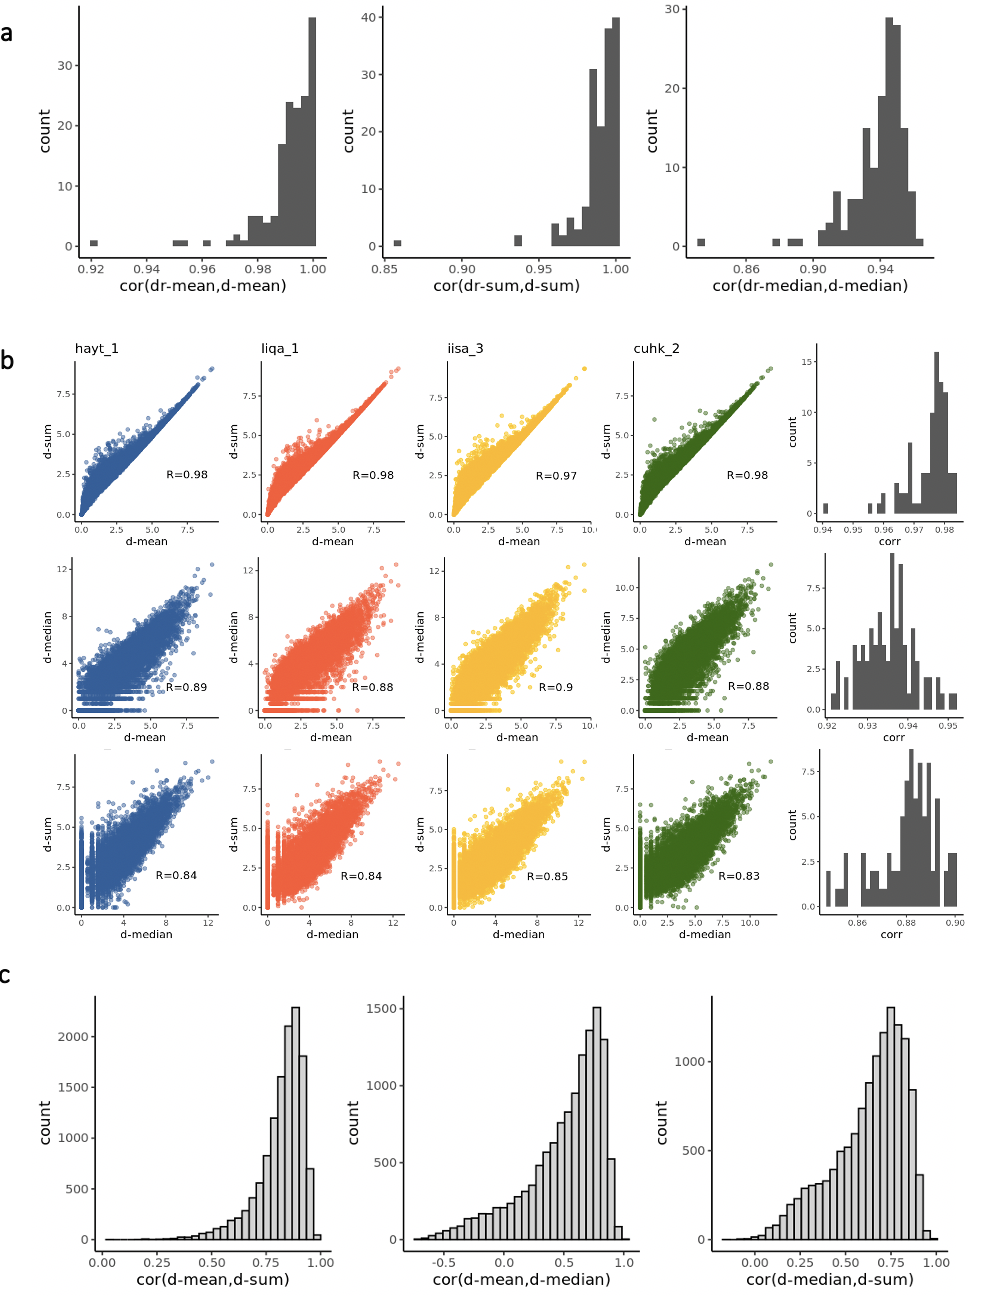
\includegraphics[width=15cm]{Appendix2/Fig/supp_aggregated_figures_d.png}
    \caption[Comparison of `d' aggregated measures]{\textcolor{blue}{\textbf{Comparison of `d' aggregated measures.}\\
    (a) Histograms of correlations between `dr' and `d' aggregation measures, for each of mean, sum, median.
    (b,c) Similar to \textbf{Fig. \ref{suppl_fig:aggregation_comparison_dr}}, panels a and b, but across `d' aggregation methods (instead of `dr'; the same donors are considered).}}
    \label{suppl_fig:aggregation_comparison_d}
\end{figure}

\begin{figure}[h]
    \centering
    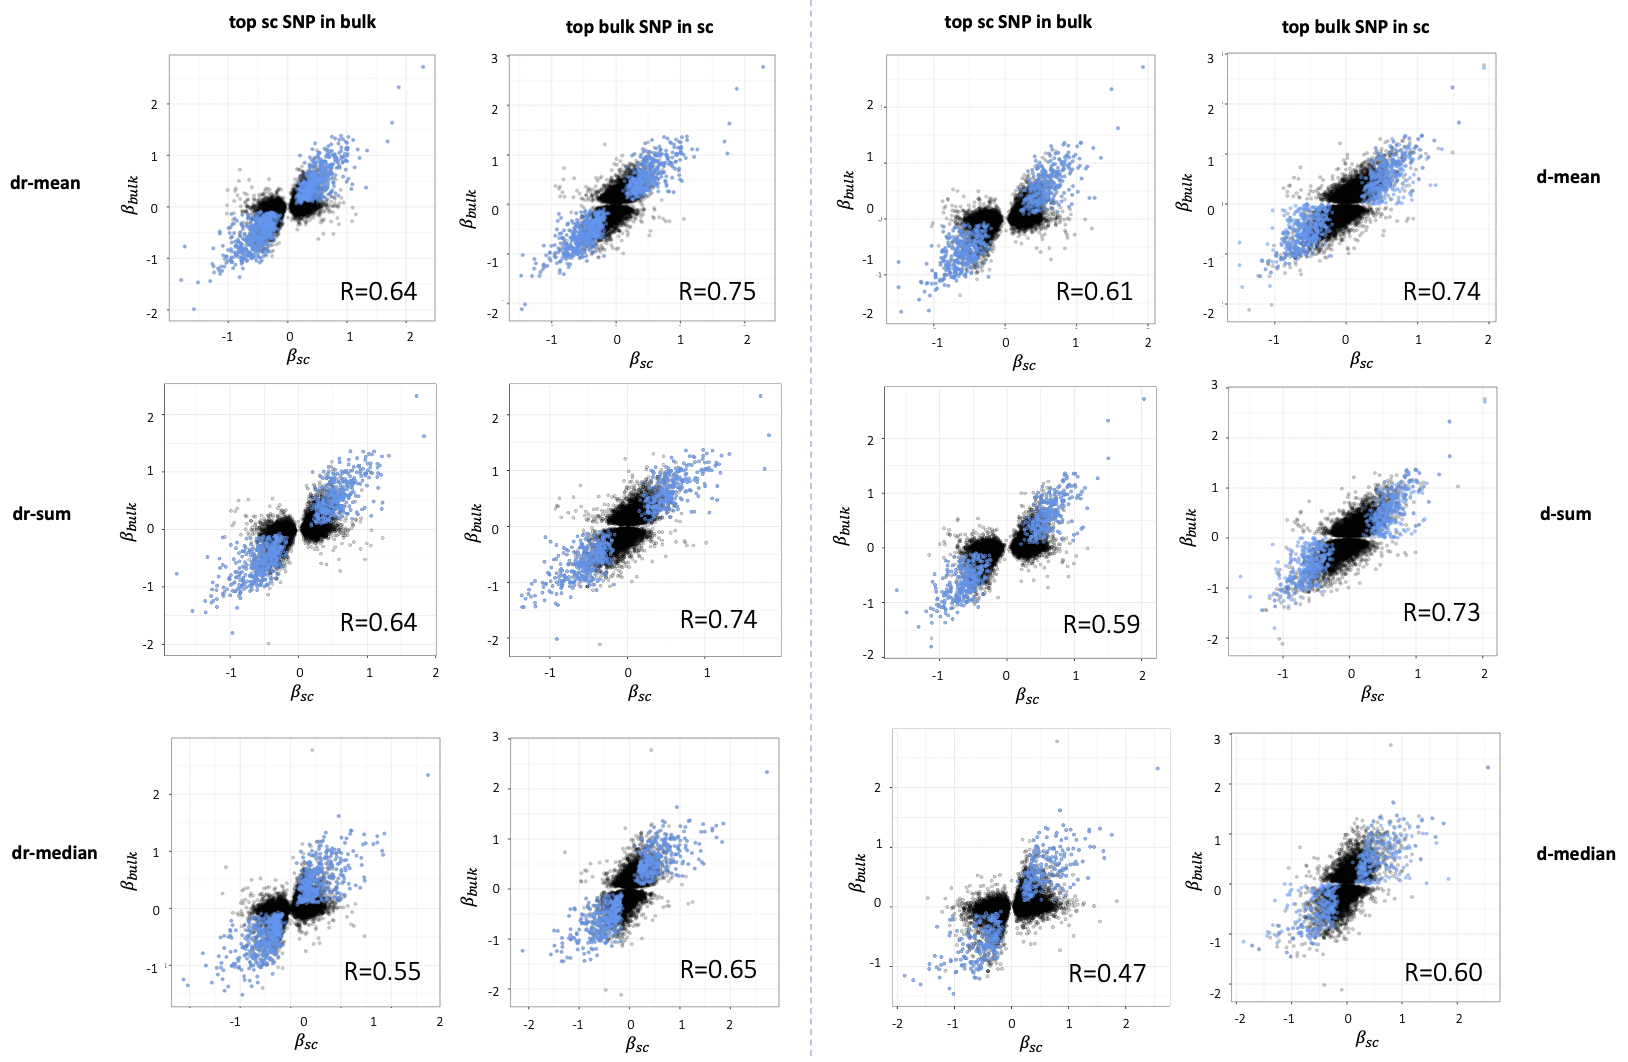
\includegraphics[width=16cm]{Appendix2/Fig/supplement_sc_vs_bulk.png}
    \caption[Comparison of results between single cell and bulk iPSC eQTL]{\textcolor{blue}{\textbf{Comparison of results between single cell and bulk iPSC eQTL.}\\
    Scatter plots of eQTL effect sizes obtained when testing association of iPSC eQTL discovered using single cell (SmartSeq2) and bulk RNA-seq.
    The bulk eQTL results considered are obtained using all samples available (`a-bulk')
    The same set of n=12,720 genes that were assessed in all maps are considered.
    First two columns, `dr'-aggregations (dr-mean, dr-sum, dr-median; aggregated at donor and sequencing run). 
    Left, top SNP per gene (such that there are exactly as many points as there are genes) from the single cell data (`discovery set'; x axis) in bulk results (`replication set'; y axis). 
    Right, vice versa (i.e. top SNP per gene in bulk results (now `discovery set' y axis), in single cell results, now `replication set', x axis).
    In blue, for each pair of sets of results are the `replicated' eQTL, i.e. eQTL at FDR<5\% in the discovery set, replicated in the replication set (FDR<10\% and same direction of effect; consistently with the results presented in \textbf{section \ref{sec:best_practice}}).
    Third and fourth columns, same as first two but for `d' methods, i.e. d-mean, d-sum, d-median (aggregated at donor level).}}
    \label{suppl_fig:sc_vs_bulk}
\end{figure}

\begin{figure}[h]
    \centering
    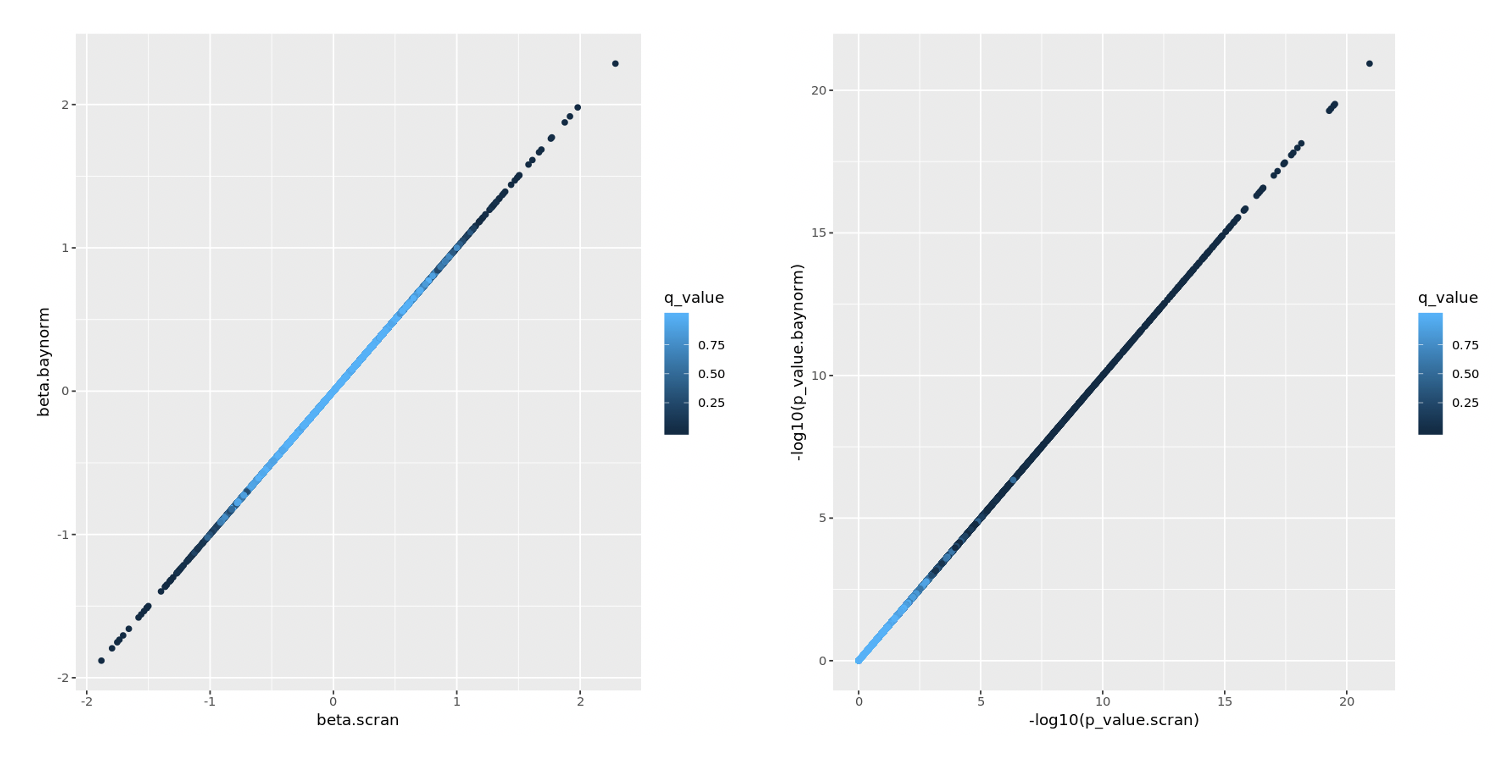
\includegraphics[width=16cm]{Appendix2/Fig/suppl_scran_vs_baynorm.png}
    \caption[Correlation of results between scran and bayNorm normalisation]{\textbf{Correlation of results between scran and bayNorm normalisation.}\\
    Related to results from \textbf{Table \ref{tab:egenes}}.
    Scatter plots of eQTL effect sizes (left) and p values (right) obtained when testing association of iPSC single cell eQTL discovered using dr-mean as aggregation method and after normalising counts using two alternative methods: scran/scater \cite{mccarthy2017scater} (x axis) and bayNorm \cite{tang2020baynorm} (y axis).}
    \label{suppl_fig:scran_vs_baynorm}
\end{figure}

\clearpage

\section{Additional results for Chapter 4}

\begin{figure}[h]
    \centering
    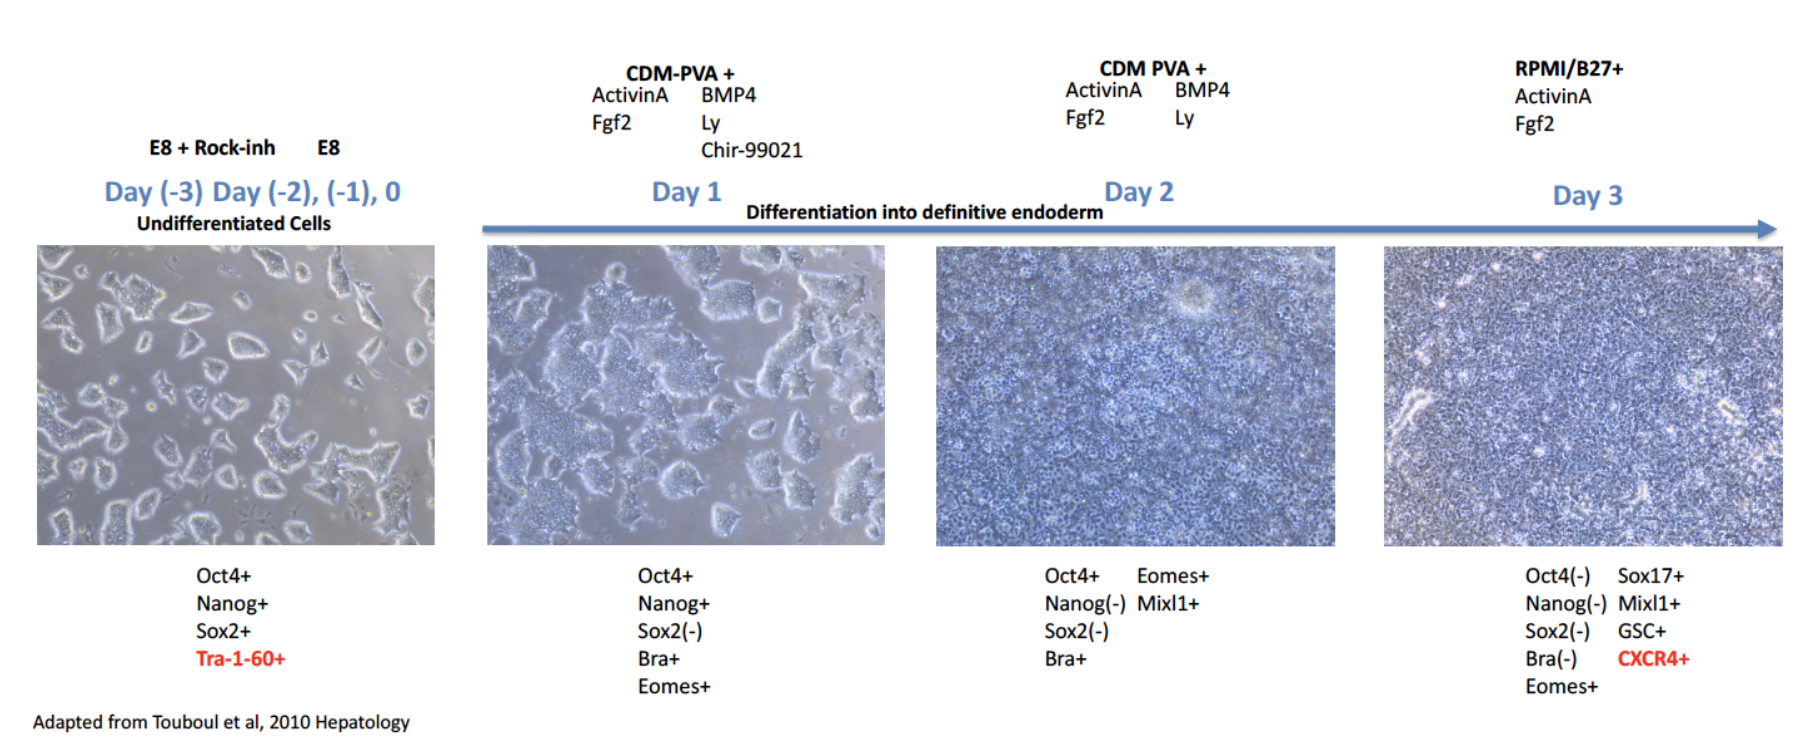
\includegraphics[width=16cm]{Appendix2/Fig/suppl_protocol.png}
    \caption[Endoderm differentiation protocol]{\textbf{Endoderm differentiation protocol.}\\
    Adapted from Touboul \textit{et al.} \cite{touboul2010generation}.
    Related to \textbf{Chapter \ref{chapter4}, section \ref{sec:endodiff_summary}}.
    Schematic representation of the chemically defined protocol used to initiate differentiation towards  definitive endoderm. 
    Tra-1-60 and CXCR4 are canonical cell surface markers of pluripotent and definitive endoderm stages, respectively, which were used to sort live cells by differentiation stage. }
    \label{suppl_fig:endodiff_exp_protocol}
\end{figure}

\begin{figure}[h]
    \centering
    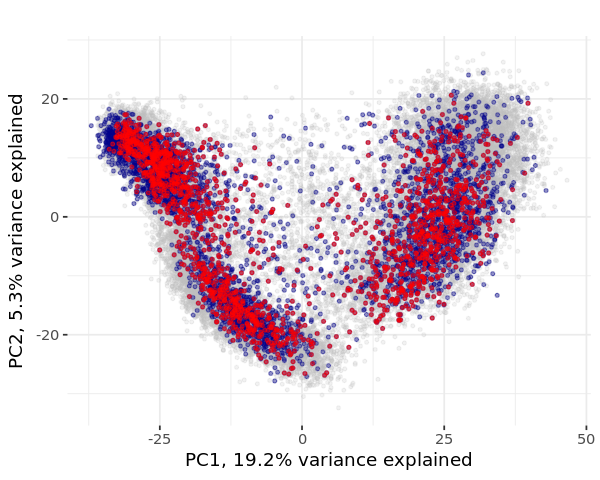
\includegraphics[width=15cm]{Appendix2/Fig/suppl_diabetes_lines.png}
    \caption[PCA of healthy and diseased cell lines]{\textbf{Comparison of expression patterns between healthy and diseased cell lines.}\\
    PCA plot (similar to \textbf{Fig. \ref{fig:endodiff_pca}}) of cells from cell lines derived from monogenic diabetes donors (red), cells from healthy donors from the same seven experiments (dark blue), against the background of all cells (grey). }
    \label{suppl_fig:pca_diabetes_lines}
\end{figure}

% FACS?

\clearpage

\section{Additional results for Chapter 5}

\begin{figure}[htb!]
    % \centering
    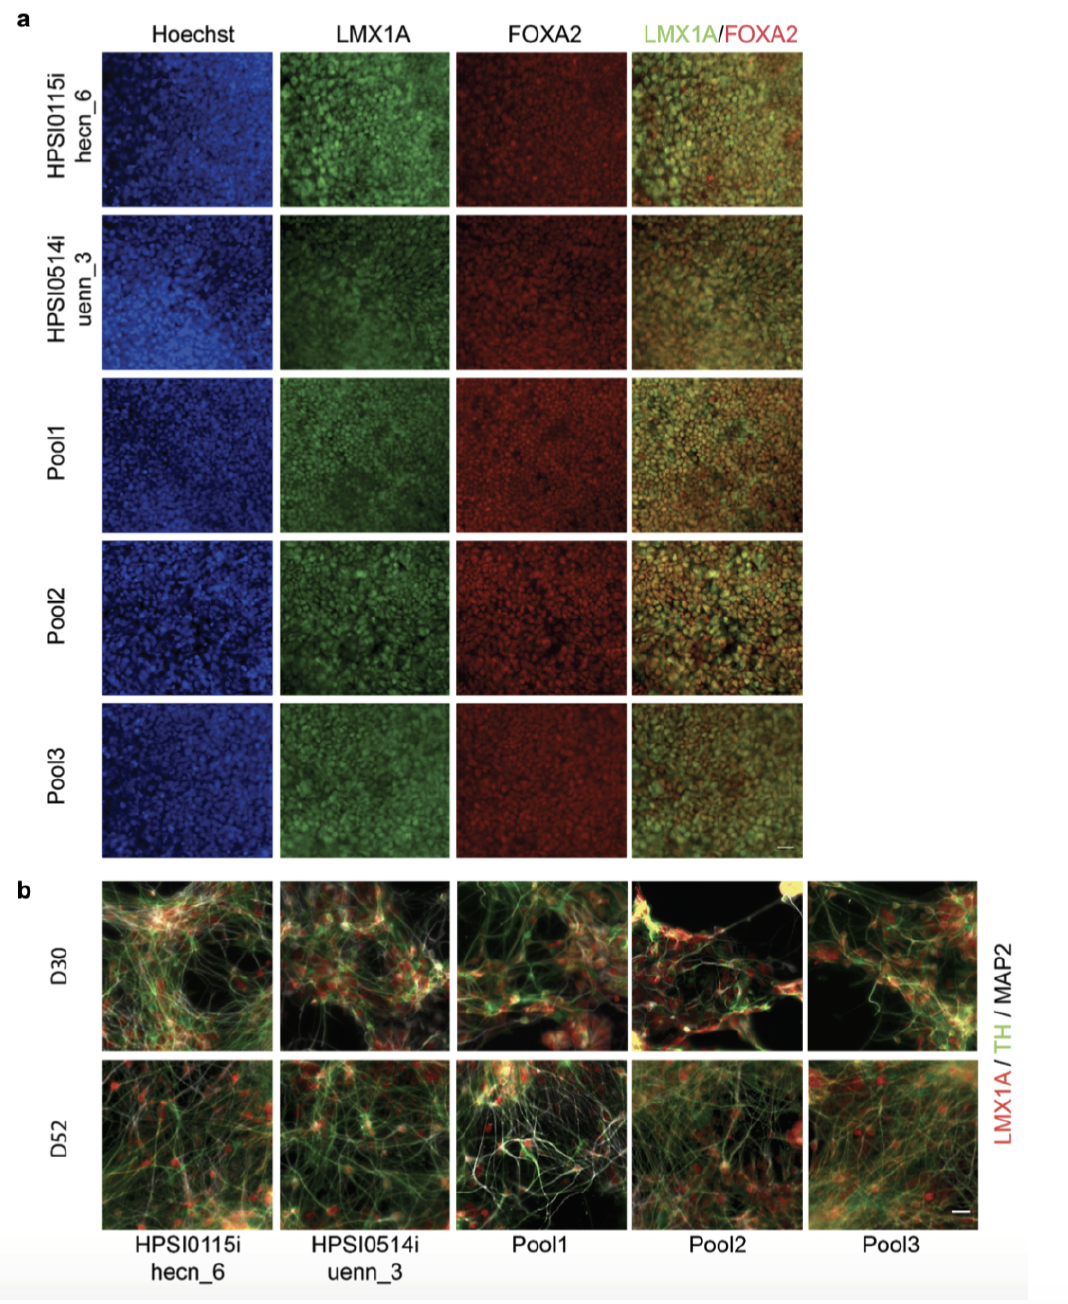
\includegraphics[width=14.5cm]{Appendix2/Fig/suppl_neuroseq_immunostaining.png}
    \caption[Immunostaining of midbrain neural progenitors and dopaminergic neurons]{\textbf{Immunostaining of midbrain neural progenitors and DA neurons (Full legend on next page).}\\}
    \label{suppl_fig:immunostaining}
\end{figure}

\newpage

\captionsetup[figure]{list=no}
\addtocounter{figure}{-1}   
\captionof{figure}{\textbf{Immunostaining of midbrain neural progenitors and DA neurons (continued).\\}
    Figure by Julie Jerber.
    (a) Immunostaining for known midbrain progenitor markers LMX1A and FOXA2 at day 11. 
    Nuclei were counterstained with Hoechst. 
    Scale bar: 25µm. 
    (b) Immunostaining of differentiated dopaminergic neurons for  the neuronal marker MAPT2 (white) and the dopaminergic neuronal markers TH and LMX1A. 
    Scale bar: 25µm. 
    Data is shown for two example individual cell lines (HPSI0155i-hecn\_6 and HPSI0514i-uenn\_3) as well as three entire differentiation pools (Pools 1,2,3).}
\captionsetup[figure]{list=yes}

\vspace{10mm}


\begin{figure}[h]
    \centering
    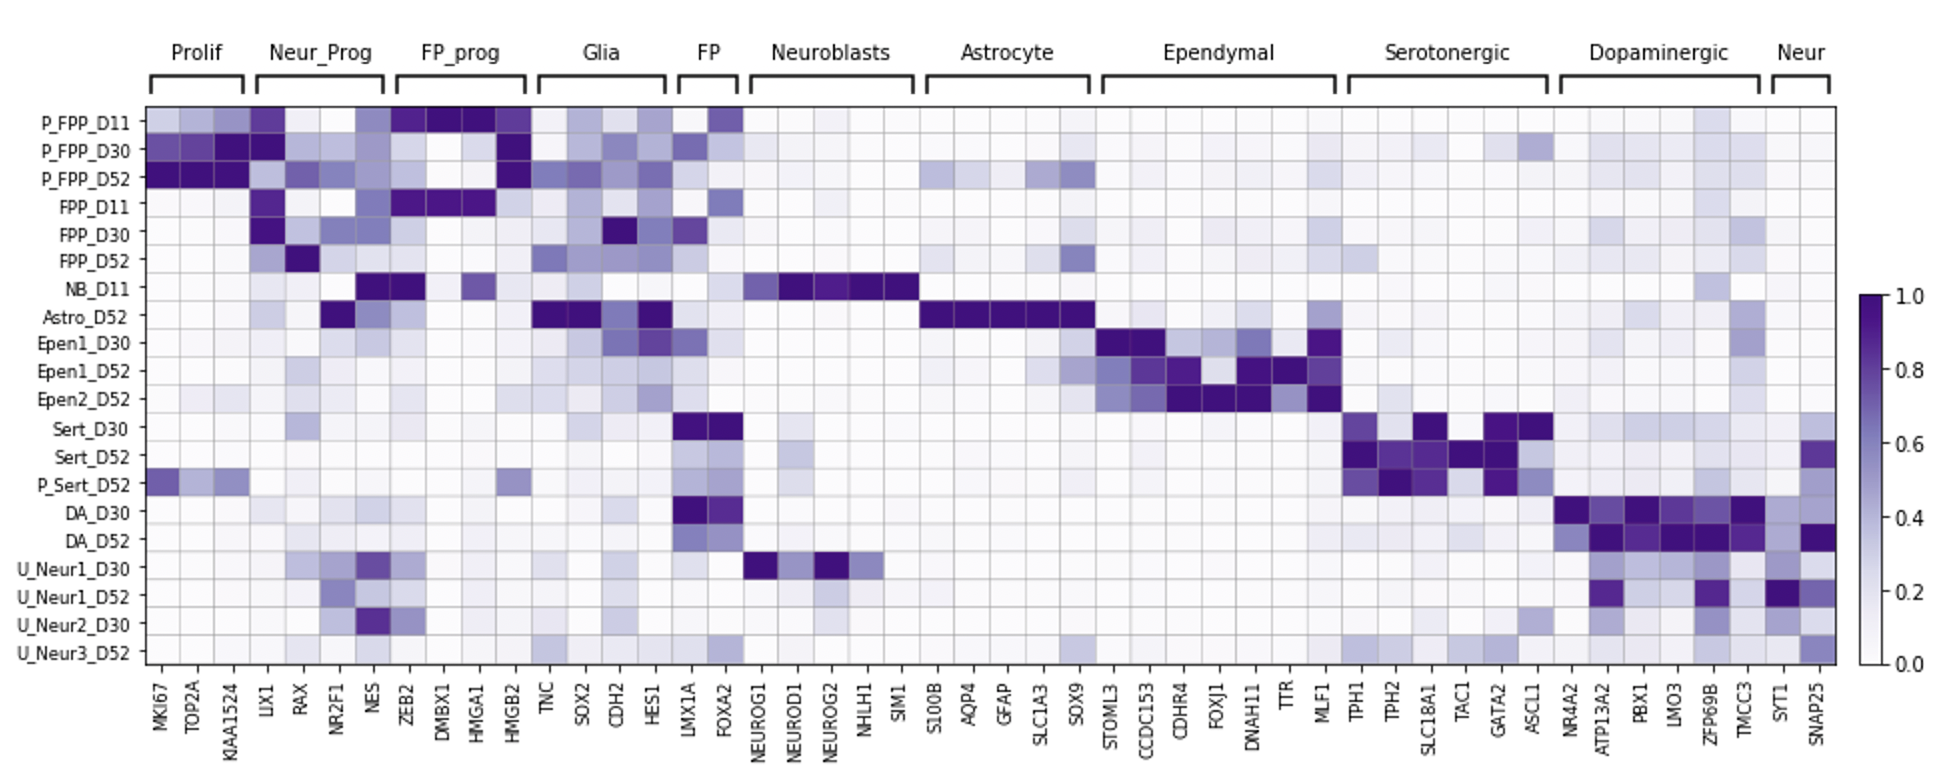
\includegraphics[width=16cm]{Appendix2/Fig/supl_neuroseq_markers.png}
    \caption[Neuronal cell type markers]{\textbf{Neuronal cell type markers}.\\
    Heat map showing the average expression of the 48 literature-curated neuronal marker genes used to annotate the identified clusters as cell types (columns) by the annotated cell types at different time points (rows, as in \textbf{Fig. \ref{fig:neuroseq_clusters}}).}
    \label{fig:suppl_celltype_markers}
\end{figure}

\begin{figure}[h]
    \centering
    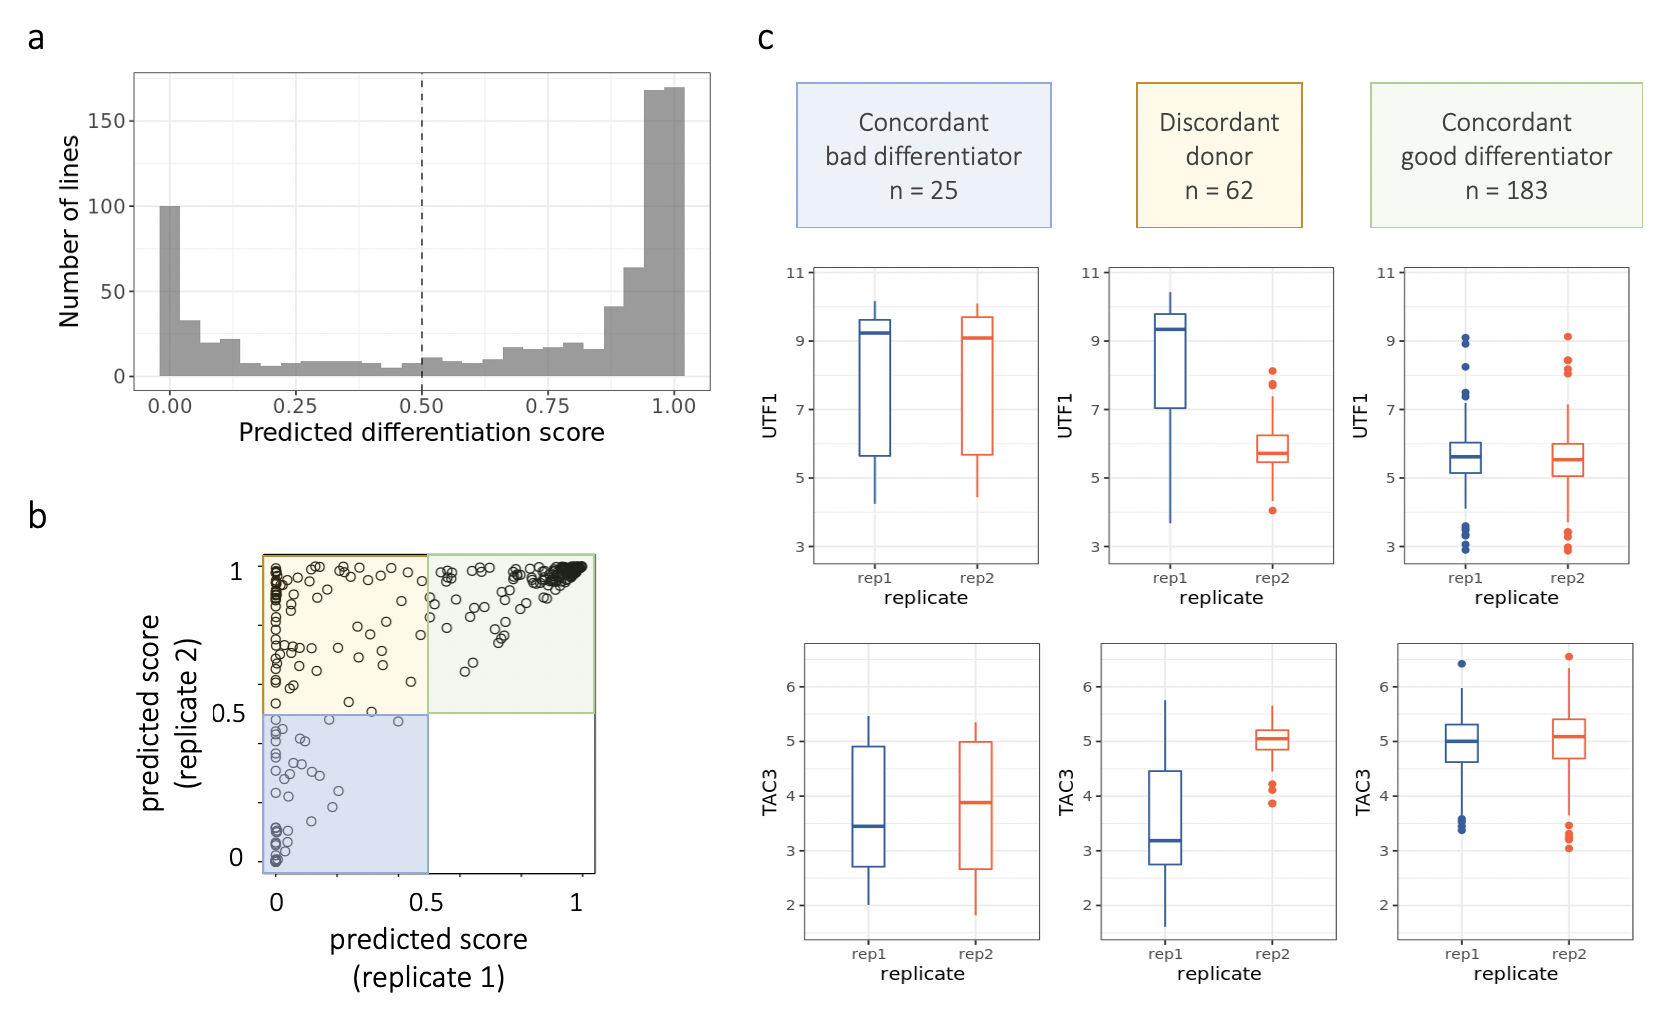
\includegraphics[width=15cm]{Appendix2/Fig/suppl_donor_effects.png}
    \caption[Predicted differentiation scores]{\textbf{Predicted differentiation scores}.\\
    Results related to \textbf{section \ref{sec:neuro_diff_eff_predictor}}.
    (a) Histogram of predicted differentiation scores across all HipSci cell lines. 
    The bimodal distribution is especially extreme in this case, and 0.5 was used as the threshold to split bad from good differentiator lines. 
    (b) Scatter plot of predicted differentiation scores for donor for which we have data for two different cell lines. Replicate1 (rep1) is chosen as the line with lower predicted score (n=270). 
    Colours indicate three categories of donors, according to whether both lines from the same donor are predicted to fail differentiation (blue), both are predicted to succeed (green), the two lines are discordant (one is predicted to successfully differentiate, but not the other, yellow). (c) Bulk RNA-seq expression of \textit{UTF1, TAC3} for the two replicate lines per donor stratified by the categorization described in (b).}
    \label{suppl_fig:predicted_scores_donors}
\end{figure}

\begin{figure}[h]
    \centering
    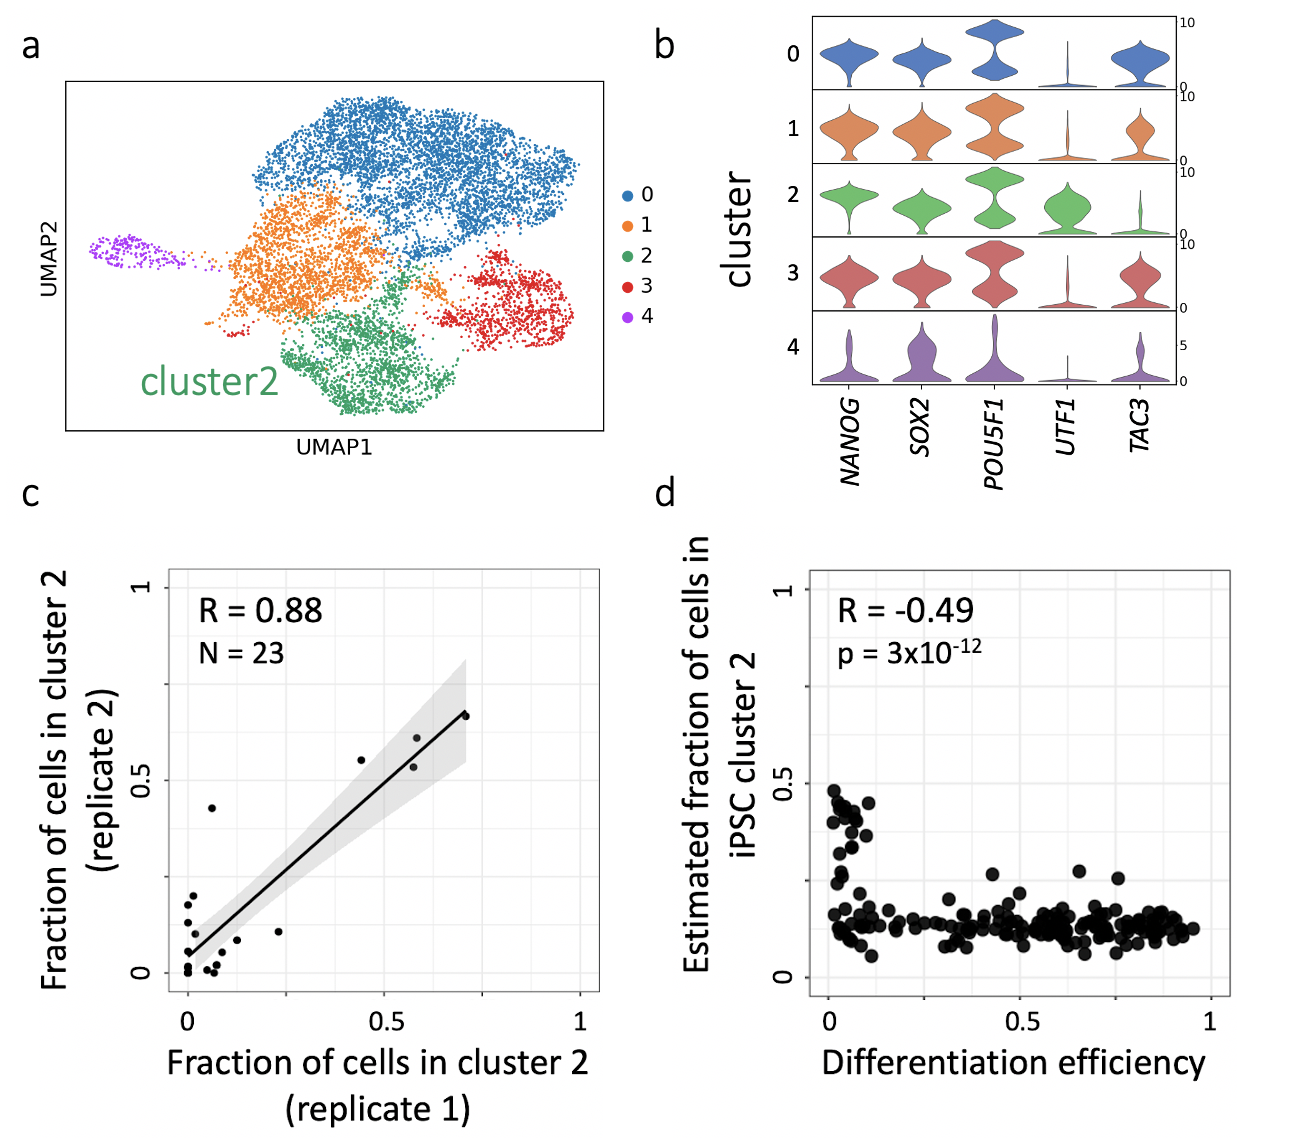
\includegraphics[width=15cm]{Appendix2/Fig/suppl_ips_cluster2.png}
    \caption[An iPSC sub-population is associated with lower differentiation efficiency]{\textbf{Re-analysis of iPSC scRNA-seq data reveals a subpopulation characterised by expression of predictive marker genes associated with lower neuronal differentiation efficiency.}\\
     (a) UMAP overview of the dataset. 
     iPSC scRNA-seq data from \cite{cuomo2020single} were re-analysed following the same batch correction and clustering steps applied to our neural differentiation data, identifying 5 clusters. 
     (b) Violin plots of gene expression for genes related to pluripotency (\textit{NANOG, SOX2, POU5F1}) and two gene markers that are respectively upregulated and downregulated in cluster 2 (\textit{UTF1, TAC3}, from \textbf{Fig. \ref{fig:neuroseq_ips_expression_signature}}). 
     (c) Scatter plot showing the proportion of cells assigned to cluster 2 between replicates (n=23). 
     (d) Scatter plot between the proportion of cells assigned to cluster 2 (y axis) and differentiation efficiency (x axis) similar to \textbf{Fig \ref{fig:neuroseq_ips_sc_genes}}, panel c, but where we use imputed proportions of cluster 2 cells from bulk RNA-seq available for most cell lines (n=182, out of 199 lines for which we have day 52 data and thus a measure of neuronal differentiation efficiency).}
    \label{suppl_fig:ipsc_cluster2}
\end{figure}


\begin{figure}[h]
    \centering
    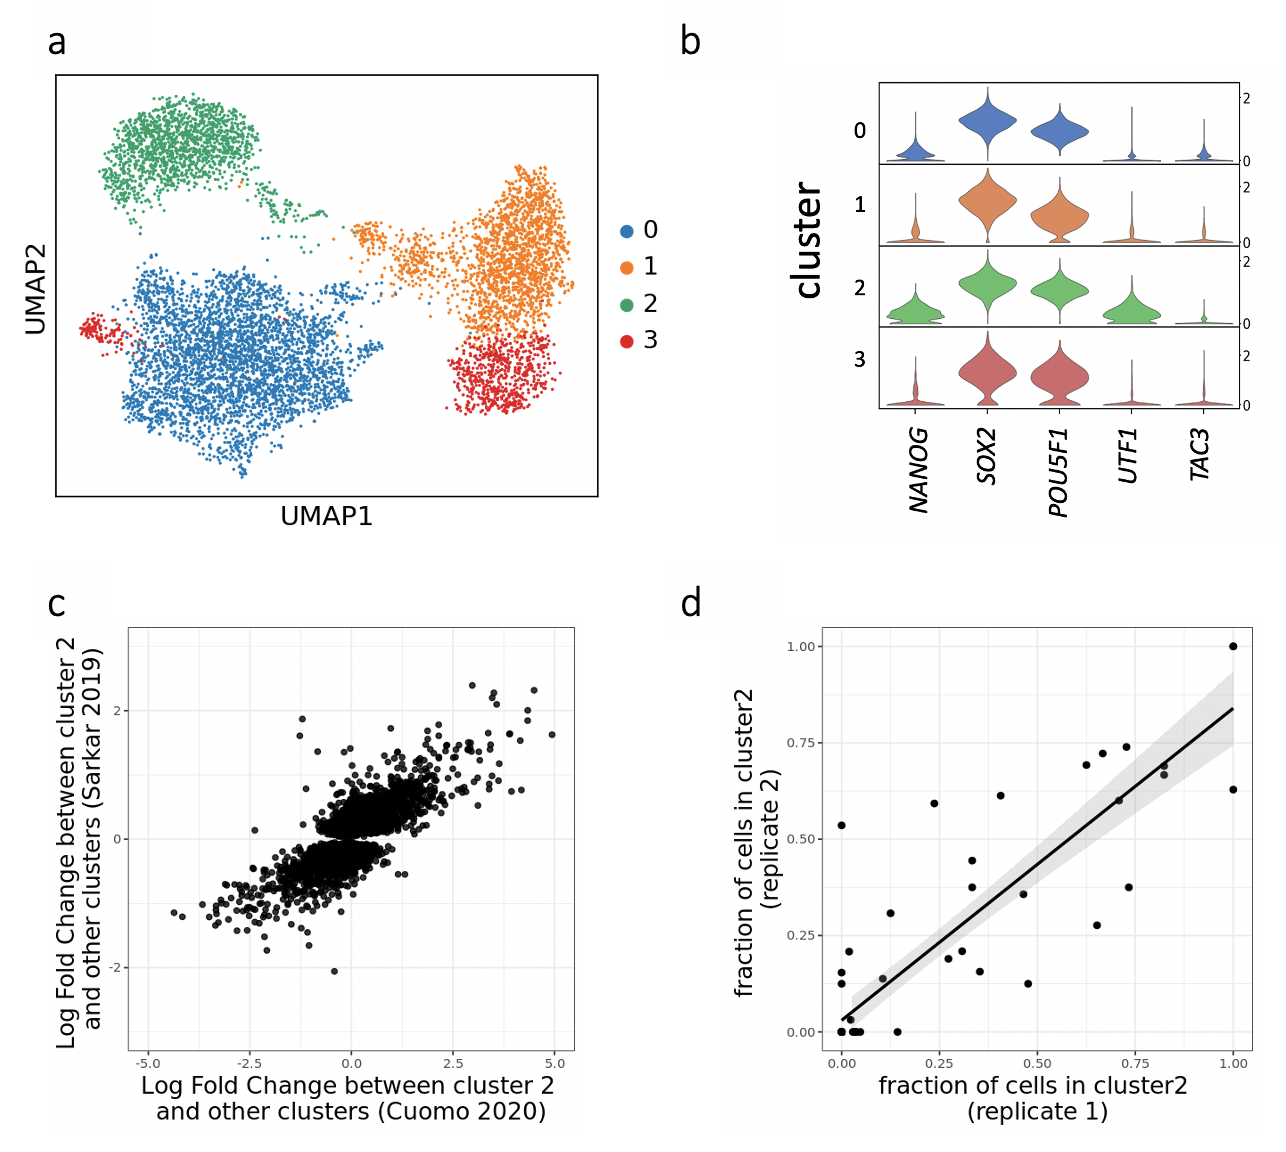
\includegraphics[width=15cm]{Appendix2/Fig/suppl_ipsc_cluster2_sarkar.png}
    \caption[Analysis of a single cell iPSC dataset from Sarkar \textit{et al.}]{\textbf{Analysis of a single cell iPSC dataset from Sarkar \textit{et al.}}\\
    Similar to \textbf{Fig. \ref{suppl_fig:ipsc_cluster2}}.
    (a) UMAP overview of the dataset. 
    iPSC scRNA-seq data from \cite{sarkar2019discovery} were re-analysed following the same data normalisation and clustering steps applied to our neural differentiation data, identifying 4 clusters. 
    (b) Violin plots of gene expression for genes related to pluripotency (\textit{NANOG, SOX2, POU5F1}) and a subset of markers of the cluster 2 population (\textit{UTF1, TAC3}). 
    (c) Scatter plot showing the proportion of cells assigned to cluster 2 between replicates (n=59). 
    (d) Expression log fold change between cluster 2 and all other clusters from \cite{cuomo2020single} compared to the same between cluster 2 and the rest from \cite{sarkar2019discovery}. 
    Shown are all 5,397 DE genes between cluster 2 and all other clusters from Sarkar \textit{et al}. (FDR < 0.05).}
    \label{suppl_fig:ipsc_cluster2_sarkar}
\end{figure}

\begin{figure}[h]
    \centering
    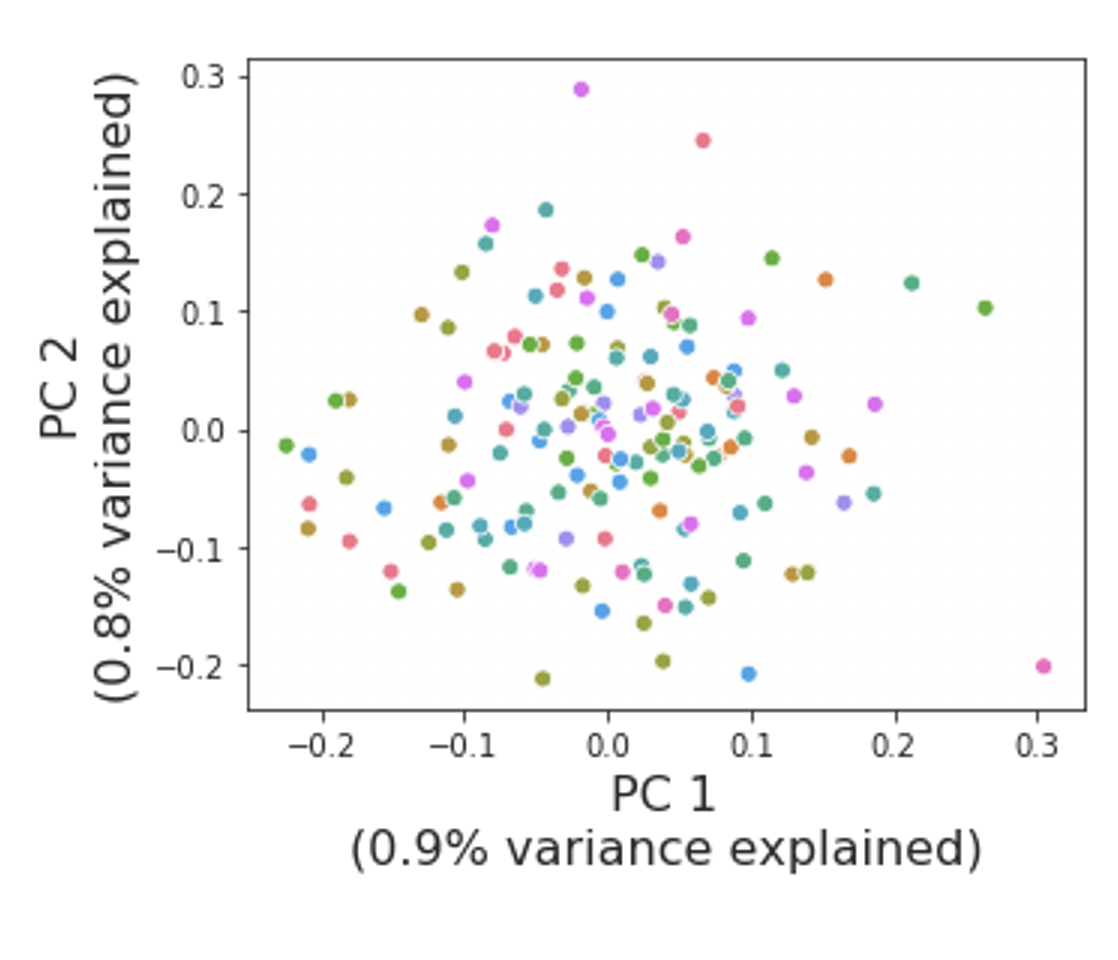
\includegraphics[width=14cm]{Appendix2/Fig/suppl_pop_struct_pc.png}
    \caption[Absence of population structure]{\textbf{Absence of population structure}.\\
    Principal component (PC) decomposition of the kinship matrix (calculated using PLINK \cite{purcell2007plink}) across all cell lines included in the study described in \textbf{Chapter \ref{chapter5}}, coloured by batch.}
    \label{suppl_fig:no_pop_struct}
\end{figure}

% cell lines from same donor prediction efficiency
